\documentclass[11pt]{article}

\usepackage{float}
\usepackage{hyperref}
\usepackage{fullpage}
\usepackage{verbatim}
\usepackage{moreverb}
\usepackage{graphicx}
\usepackage{parskip}
\usepackage{amsmath}
\usepackage[toc,page]{appendix}

\usepackage{minted}
\let\verbatiminput=\verbatimtabinput
\def\verbatimtabsize{4\relax}

\begin{document}
\title{EE 241B HW1 Writeup}

\author{Vighnesh Iyer}
\date{}
\maketitle

\tableofcontents

\section{Models - MOSFET Characterization}

We are using a 32nm LP CMOS process for this class. The devices being characterized are \verb|n105| and \verb|p105| (TT corner) with a nominal supply voltage of 1.05V.

\subsection{Threshold Voltages}
We want to determine the threshold voltage $V_{th}$ for the NMOS and PMOS devices (for $V_{BS}$ = 0, $L$ = 32nm, and $W$ = 1$\mu$m), by extrapolating from the $I_DS$ vs. $V_{GS}$ curve at low $V_{DS}$. We compare the threshold voltage derived from DC sweeps to the values reported in the model file and the DC operating point analysis.

To perform this characterization, we first collect a full range of DC operating points for both transistors to make analysis easier for this entire section. The transistors' drains are connected to a variable DC supply and the transistors' gates are connected to another independent variable DC supply. The source for both transistors is held at ground (0V). We perform a nested DC analysis by sweeping $V_{DS}$ from $0 \rightarrow 1.05$V in (10mV) increments, and sweep $V_{GS}$ from $0 \rightarrow 1.05$V in (10mV) increments.

The gathered I-V curves are shown below.

\begin{figure}[H]
	\centerline{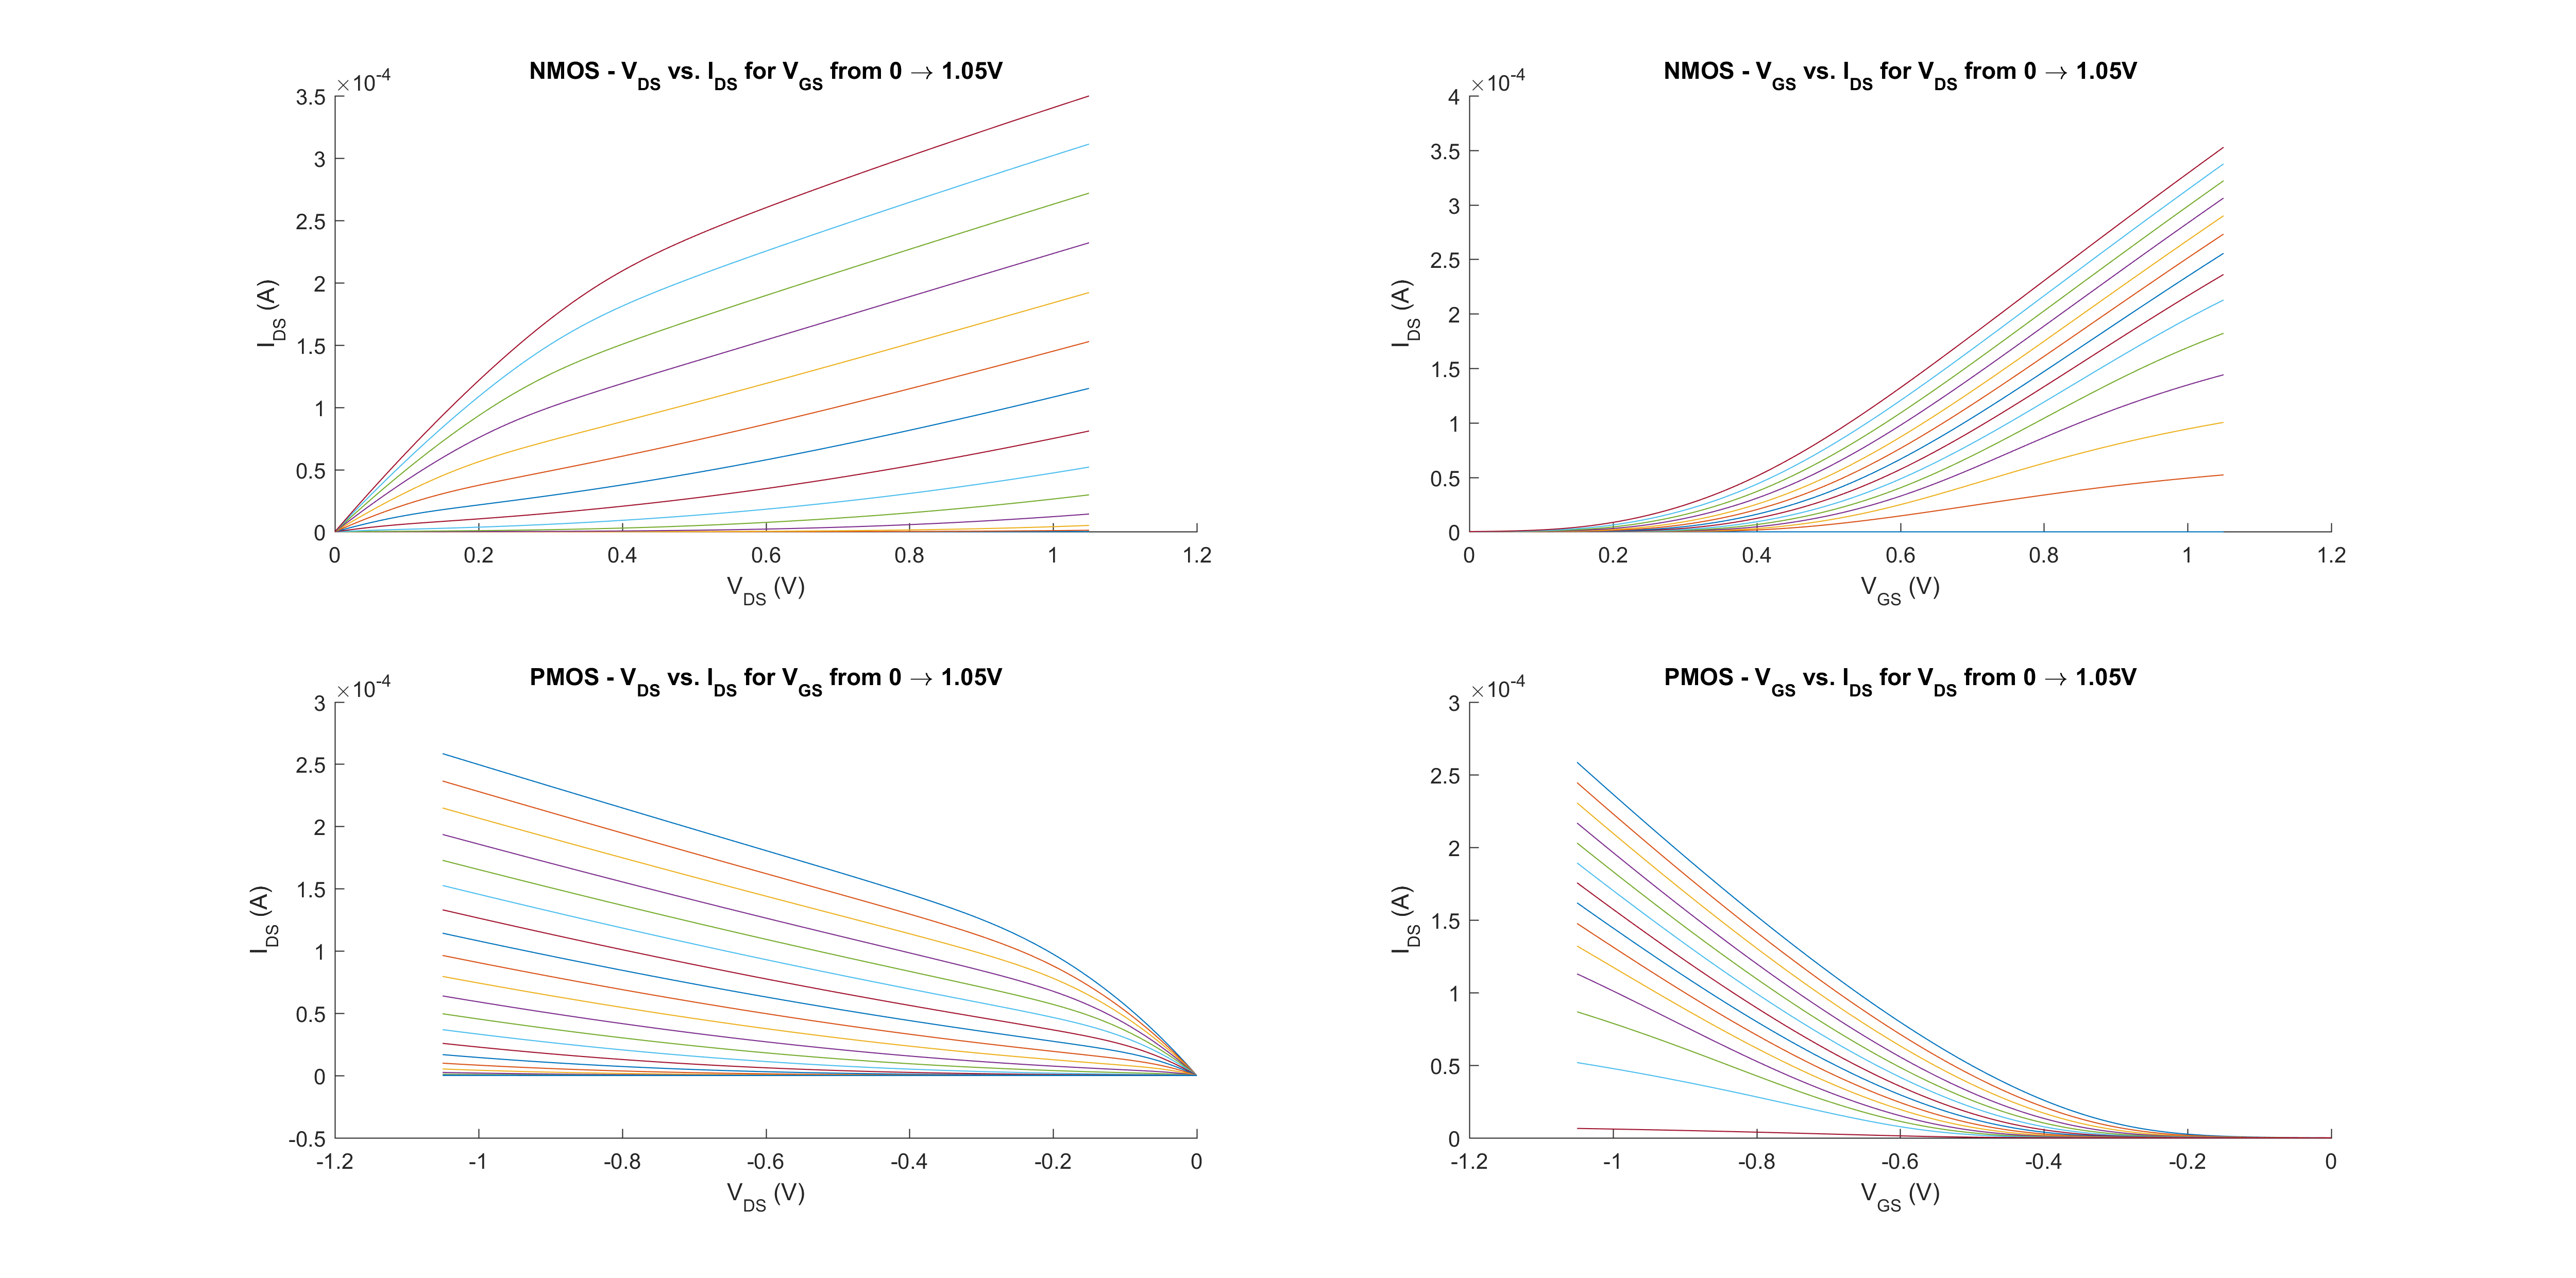
\includegraphics[width=\textwidth+5cm]{images/dc_curves.png}}	
\end{figure}

From the DC OP analysis, $V_{th}$ of the NMOS is reported to be 324.4 mV, and the $V_{th}$ of the PMOS is reported to be -208.1 mV. From the model files the NMOS $V_{th}$ is 370 mV, and the PMOS $V_{th}$ is -213 mV.

To extract the threshold voltage from the I-V curves, we extrapolate the $V_{GS}$ vs $I_{DS}$ curves for a low value of $V_{DS}$ to keep the transistor in the linear region of operation. Then we fit a linear curve to the points where $V_{GS}: [0.4, 0.6]$ for each $V_{DS}$ curve. We treat the x-intercept of those linear curves as the $V_{th}$ of the transistor for the given value of $V_{DS}$. This method is shown for NMOS and PMOS transistors.

\begin{figure}[H]
	\centerline{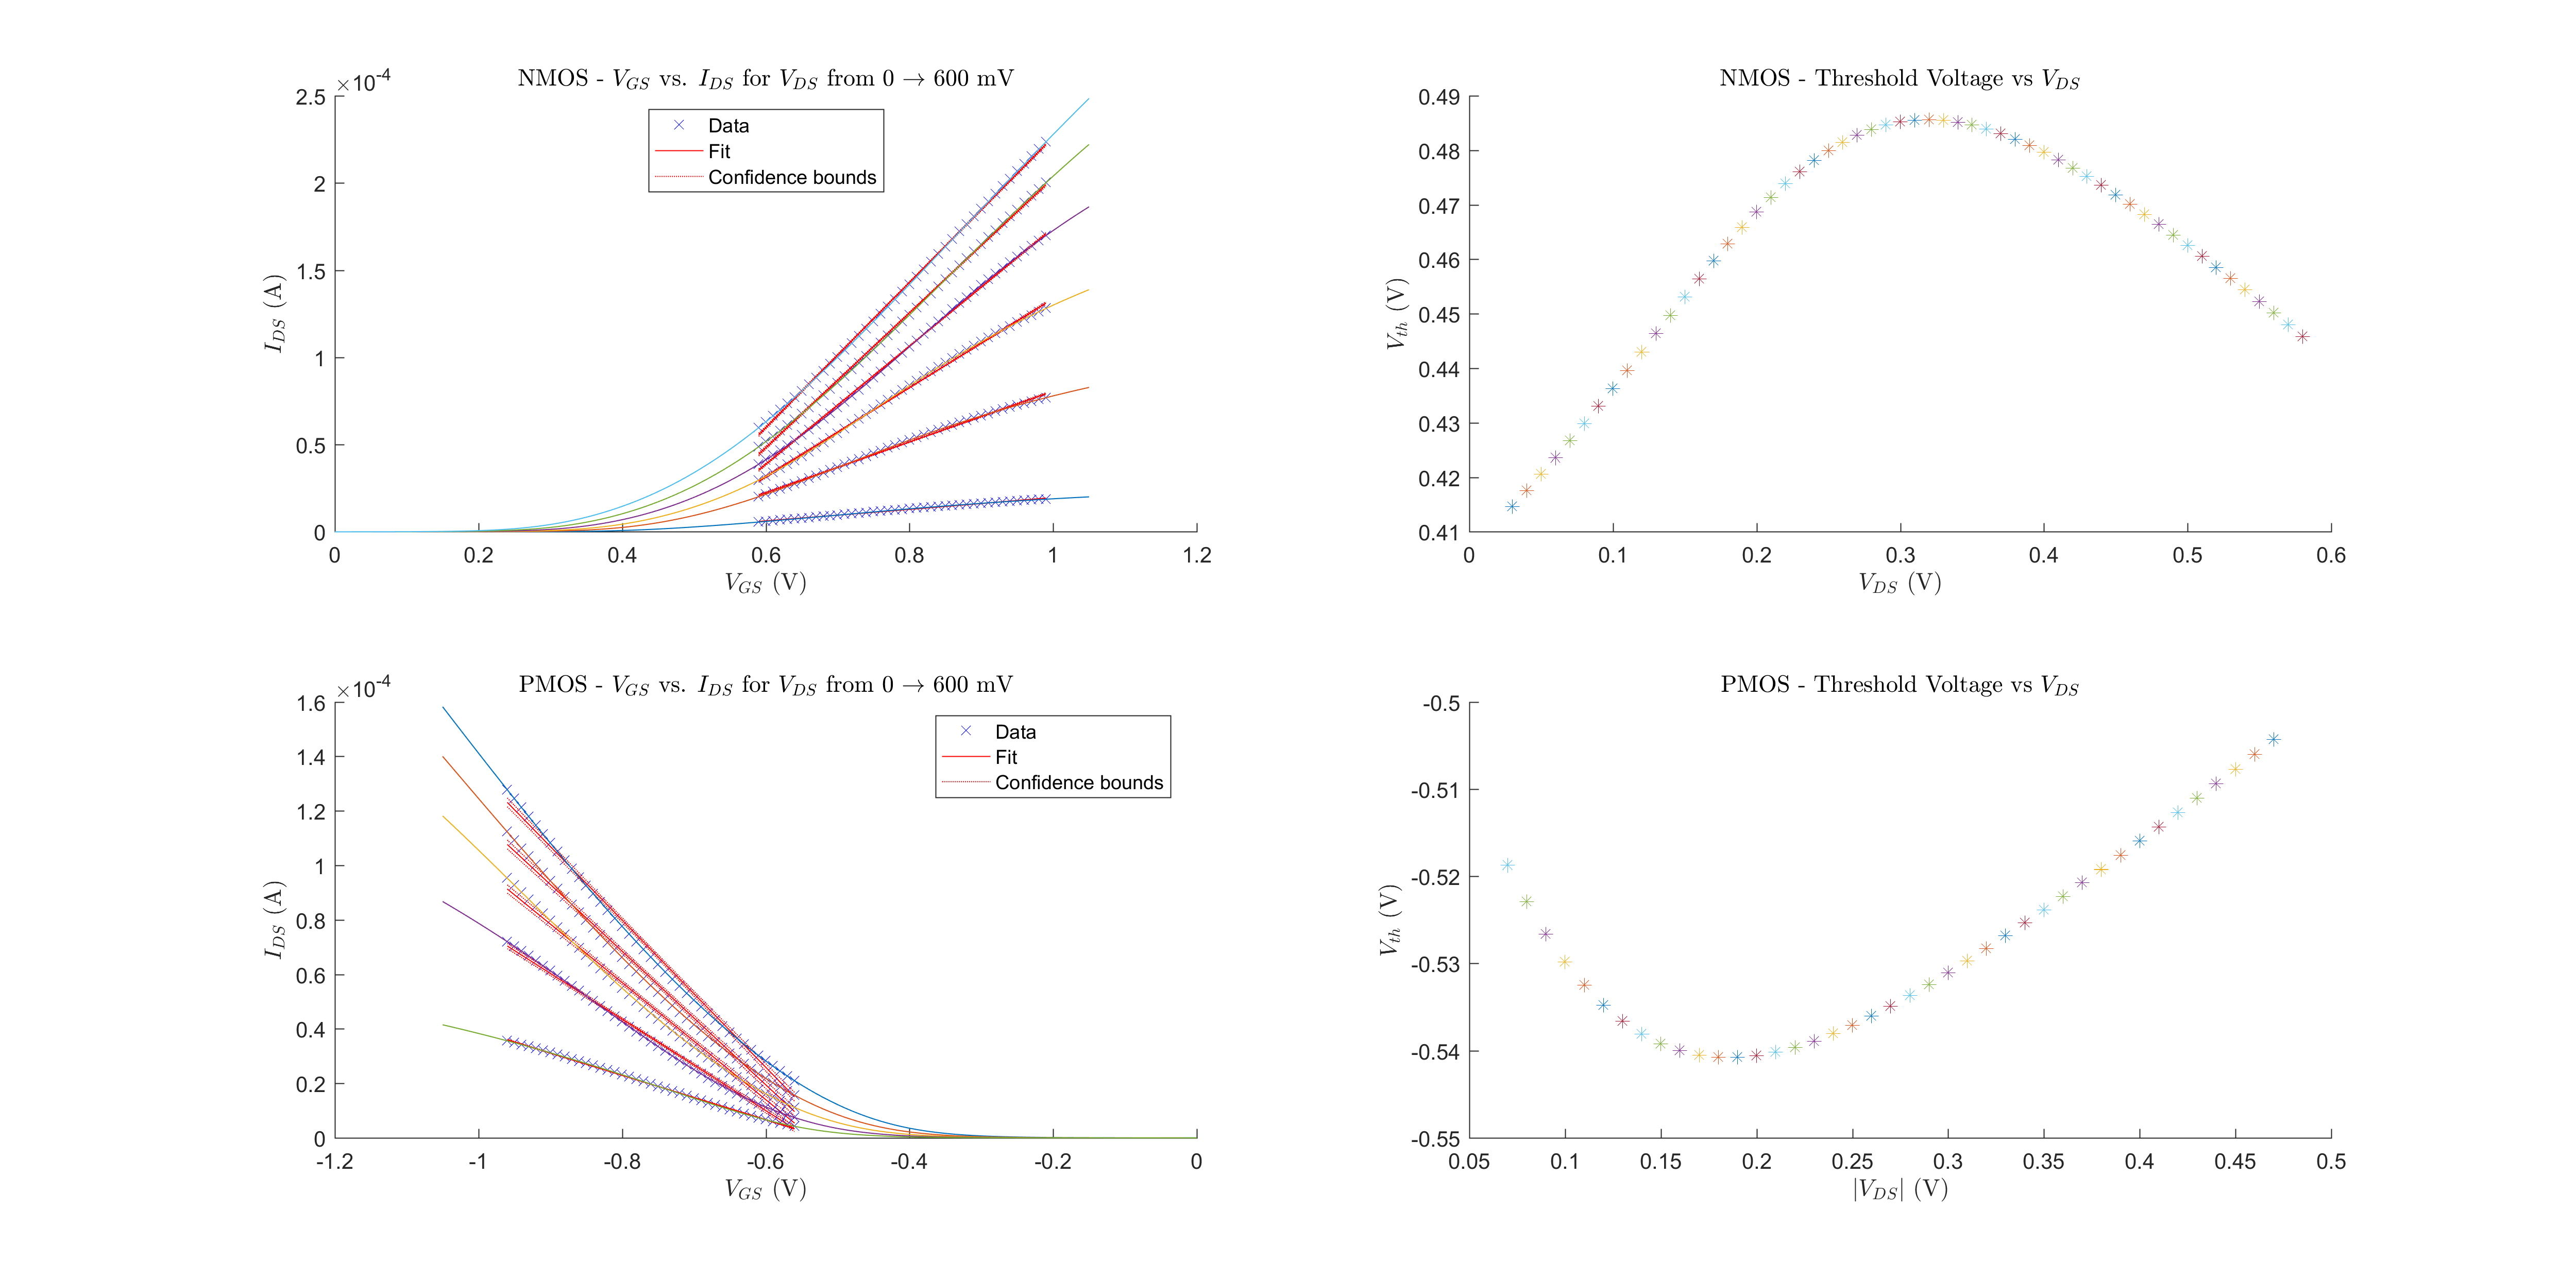
\includegraphics[width=\textwidth+5cm]{images/threshold_voltage.png}}	
\end{figure}

The images on the left side show the linear fit to each curve, while the images on the right side show the extrapolated $V_{th}$ for each $V_{DS}$ curve. As expected, with increased $V_{DS}$ the threshold voltage improves for both devices. 

The extrapolated results for the NMOS match the model files and the DC operating point measurement well. However, the PMOS threshold voltage is off by around 100 mV.

\section{Fit Velocity Saturation Model}
In class, we use this model for $I_{DSat}$:

\begin{equation*}
	I_{DSat} = \frac{W}{L} \frac{\mu_{eff} C_{ox} E_C L}{2} \frac{(V_{GS} - V_{th})^2}{(V_{GS} - V_{th}) + E_C L}
\end{equation*}

We want to find the values of $E_C L$ that best fit the NMOS and PMOS characteristics. We will use the $V_{th}$ value from the previous section. We take the case of the $V_{DS}$ curve where $V_{DS} = V_{DD}$ to keep the transistors fully saturated and we sweep $V_{GS}$. We then fit our simulation data in saturation where $V_{GS} > V_{th}$ to this model with $E_C L$ and $k'$ as free variables.

\newpage
\appendix
\section{PMOS/NMOS DC Characterization SPICE Sim} \label{dc_characterization_spice}
\begin{minted}{text}
Sweep of V_GS with constant V_DS for N-MOSFET
.lib '/home/ff/ee241/synopsys-32nm/hspice/saed32nm.lib' TT
vds vds gnd 1.05
vgs vgs gnd 1.05 
x1 vds vgs gnd gnd n105 (w=1u l=32n)

.op
.dc vgs 0 1.05 10m vds 0 1.05 10m

.option post=2 nomod
.end
\end{minted}

\section{}

\end{document}